\documentclass[12pt, oneside]{article}
\usepackage{geometry}
\usepackage[utf8]{inputenc}
\usepackage{setspace}
\usepackage{times}
\usepackage{url}
\urlstyle{same}
\usepackage{multirow}
\usepackage[usegeometry]{typearea}
% Useful for checking layout
% \usepackage{showframe}
\usepackage{fancyhdr}
\usepackage{blindtext}
% Indenting the first sentence after section
\usepackage{indentfirst}
% Set language
\usepackage[german]{babel}
% Abbreviations
\usepackage{glossaries}
% For big tables which span multiple pages
\usepackage{longtable}
% Images
\usepackage{graphicx}
\graphicspath{ {./images/} }
% APA Citation Style
\usepackage[natbibapa]{apacite}
% Smaller font size for captions
\usepackage[font=small,labelfont=bf]{caption}
% Table related packages
\usepackage{booktabs}


\geometry{
 a4paper,
 left=30mm,
 top=25mm,
 right=25mm,
 bottom=20mm,
 footskip=15pt,
}

\setstretch{1.3} % Define Line Spacing
\renewcommand{\headrulewidth}{0pt} % Remove footer line

\pagestyle{fancy} % Allow for customizing header and footer
% Customize footer for page number location
\fancyhf{}
\fancyfoot{}
\fancyhead[R]{Yannick Hutter}
\fancyhead[L]{Exposé}
\fancyfoot[R]{\thepage}



 \makeglossaries

 \newglossaryentry{dsr}
 {
     name=DSR,
     description={Design science Research}
 }
 \newglossaryentry{foph}
 {
     name=FOPH,
     description={Federal Office of Public Health}
 }
 \newglossaryentry{fhgr}
 {
     name=FHGR,
     description={Fachhochschule Graubünden}
 }
 \newglossaryentry{svi}
 {
     name=SVI,
     description={Social Vulnerability Index}
 }
 \newglossaryentry{who}
 {
     name=WHO,
     description={World Health Organisation}
 }



\begin{document}
\pagenumbering{roman}
\begin{titlepage}
	\begin{center}
		\Huge
		\textbf{Exposé}
		
		\vspace{0.5cm}
		\LARGE
		Analyse und Implementierung eines personalisierbaren Corona Dashboards für Millenials
		
		\vspace{1.5cm}
		\normalsize
		\textbf{Yannick Hutter}\\
		\textbf{Digital Business Management Klasse 18tz}\\
		\textbf{Talackerstrasse 8}\\
		\textbf{8887 Mels}\\
		\textbf{yannick.hutter@stud.fhgr.ch}\\

		
		\vfill
		Referrent: Daniel Klinkhammer\\
		Korefferent: Michael Burch\\
		
		\vspace{0.8cm}
		
		
		Digital Business Management\\
		Fachhochschule Graubünden\\
		Mels, April 2022
	\end{center}
\end{titlepage}



\tableofcontents
\listoffigures
\listoftables

\clearpage
\printglossaries



\clearpage
\pagenumbering{arabic}
\setcounter{page}{3}

\section{Einleitung}
Die Coronavirus-Pandemie (fortlaufend als Corona bezeichnet) hat in grossen Teilen der Welt seine Spuren hinterlassen. So geht gemäss dem \Gls{foph} hervor, dass im Zeitraum vom 24.02.2020 bis zum 10.03.2022 mehr als 3 Millionen Ansteckungen in der Schweiz, sowie im Liechtenstein verzeichnet worden sind ~\citep{FOPH.13.03.2022}. Ein wichtiges Mittel zur Kommunikation mit der Bevölkerung sind hierbei Datenvisualisierungen, insbesondere Dashboards.
Der Begriff Dashboard kommt ursprünglich aus dem Englischen und bezieht sich auf das Armaturenbrett des Autos, wo alle relevanten Informationen übersichtlich auf einem Blick ersichtlich sind ~\citep{Duden.18.04.2022}.\\

Auch bei Corona wurde eine Vielzahl von Dashboard Visualisierungen erstellt, auf denen die wichtigsten Indikatoren der Pandemie wie Fallzahlen etc. ersichtlich sind. Ein Beispiel hierzu, welches versucht ein globales Bild wiederzugeben, ist das WHO Coronavirus Dashboard ~\citep{WHO.23.04.2022}. Auf diesem Dashboard sind Ansteckungszahlen, Todesfälle sowie Impfquoten ersichtlich. Das eine weltweite Organisation wie \Gls{who} sich um die Erstellung von Datenvisualisierungen zur Corona Thematik bemüht, soll aufzeigen, wie wichtig Visualisierungen und insbesondere Dashboards geworden sind.
\clearpage

\section{Forschungsfrage}
Die Landschaft der Corona Datenvisualisierungen ist sehr breit gestrickt und umfasst unterschiedlichste Repräsentanten von Visualisierungsarten. Nebst den einzelnen Visualisierungen wie Liniendiagramme, welche den zeitlichen Verlauf von einzelnen Variablen (z.Bsp Corona Ansteckungszahlen) aufzeigen, werden diese aber auch in Form von Dashboards zusammengefasst. Eine grosse Anzahl dieser Dashboards sind jedoch  allgemein gehalten und fokussieren sich auf die breite Öffentlichkeit oder Datenanalysten. Auch gibt es von der Nutzerseite her \textbf{wenig Personalisierungsmöglichkeiten}. Anpassungen an bereits erstellten Dashboards sind in der Regel nicht vorgesehen. Interessant in diesem Kontext ist es zu untersuchen, wie sich eine spezifische Nutzergruppe ein personalisierbares Corona Dashboard vorstellt und welche \textbf{Informationen} beziehungsweise \textbf{Visualisierungsarten} von Relevanz sind. Aufgrund dieser explorativen Fragestellung ergibt sich folgende übergeordnete Forschungsfrage:


\begin{center}
\textbf{Wie stellen sich Millennials ein personalisierbares Corona Dashboard vor?}
\end{center}

Um diese Forschungsfrage abzudecken, wurden folgende untergeordnete Fragestellungen formuliert:

\begin{center}
\textbf{Welche Visualisierungstypen in Bezug auf Corona werden von Millennials gefordert?\\
(untergeordnete Forschungsfrage 1)}
\end{center}

\begin{center}
\textbf{Welche Informationen in Bezug auf Corona werden von Millennials gefordert?\\
(untergeordnete Forschungsfrage 2)}
\end{center}

\begin{center}
\textbf{Welche Personalisierungsmöglichkeiten in Bezug auf Dashboards werden von Millennials gefordert?\\
(untergeordnete Forschungsfrage 3)}
\end{center}

\clearpage
\section{Methodische Vorgehensweise}
\subsection{Methodik}
Da es sich bei der übergeordneten Forschungsfrage um eine Fragestellung mit explorativem Charakter handelt, wird für die Methodik das Design Science Research (\Gls{dsr}) Modell nach Peffers verwendet (siehe Abbildung 1).


\begin{figure}[ht]
	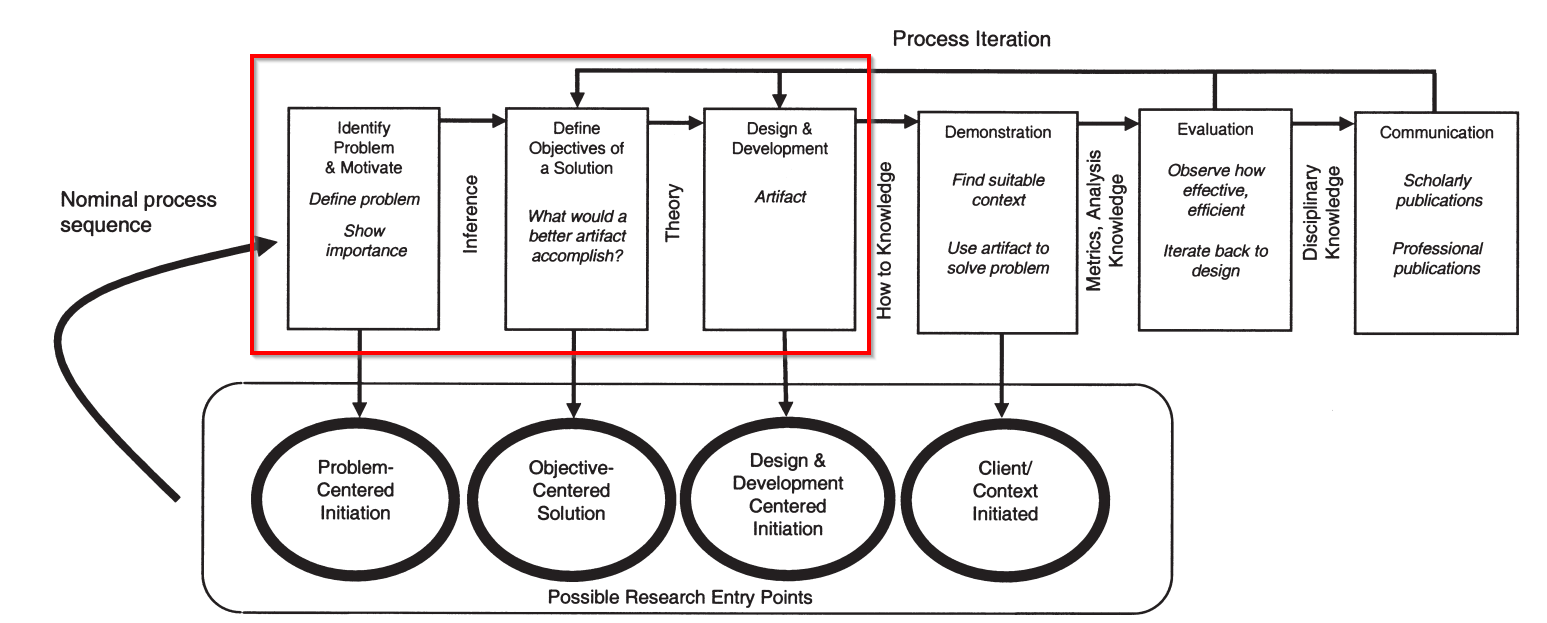
\includegraphics[width=12cm]{images/peffers_dsr_model.png}
	\centering
	\caption{DSR Modell nach Peffers ~\citep{K.Peffers.2007}}
\end{figure}

Bei diesem Modell gibt es mehrere Einstiegsmöglichkeiten (siehe \textit{Possible Research Entry Points}). Der Einstiegspunkt für die vorliegende Arbeit bildet der Punkt \textbf{Problem-Centered Initiation}. Das Problem, welches gelöst werden soll, ist die die starre Natur bestehender Corona Dashboards. Diese Dashboards lassen nach \textbf{der Erstellung für die angesprochene Zielgruppe} nicht mehr anpassen oder personalisieren. In diesem Kontext ist die Entwicklung eines Prototyps interessant, welcher die Erstellung der Dashboards \textbf{in die Hände der Zielgruppe selbst legt} und so auch Personalisierungs- und Anpassungsmöglichkeiten bietet. Dies bildet somit die Grundlage für den ersten Schritt des Models \textit{Identify Problem und Motivation}. Im zweiten Schritt \textit{Define Objective of a Solution} geht es darum, das Ziel einer möglichen Lösung aufzuzeigen. Anschliessend geht es im Schritt \textit{Design und Development} um die eigentliche Erstellung des Artefakts, was im Zuge dieser Arbeit ein High Fidelity Prototyp darstellt. In den nächsten Schritten wird die Evaluation des erstellten Prototyps, sowie die Publikation der Ergebnisse behandelt. Jedoch beschränkt sich die vorliegende Arbeit auf die Erstellung eines Prototyps aufgrund teilstrukturierter Interviews mit Millennials. Die eigentliche Evaluation des Prototyps kann im Rahmen einer weiterführenden Arbeit evaluiert werden.

\clearpage
\subsection{Vorgehen}
Eine mögliche Art der Personalisierung von Dashboards besteht darin, dass der Nutzer aus einem Katalog von Visualisierungarten (zum Beispiel Liniendiagramme welche Corona Fallzahlen darstellen) seine gewünschten Visualisierungen auszuwählen und diese frei auf dem eigenen Dashboard platzieren kann. Eine Visualisierung stellt eine gewisse \textit{Information} in einer leicht verständlichen und anschaulichen Weise dar. In einem ersten Schritt muss also die notwendige Information, welche die Grundlage für die Visualisierung darstellt, evaluiert werden. Hierzu wird das Codebook von Zhang verwendet ~\citep{YixuanZhang.2021}. Zhang untersuchte in seiner Studie \textit{Mapping the Landscape of COVID-19 Crisis Visualizations} eine Vielzahl von unterschiedlichen Corona Datenvisualisierungen und teilte diese in verschiedene Nachrichtenkategorien ein (siehe Abbildung 2).

\begin{figure}[ht]
	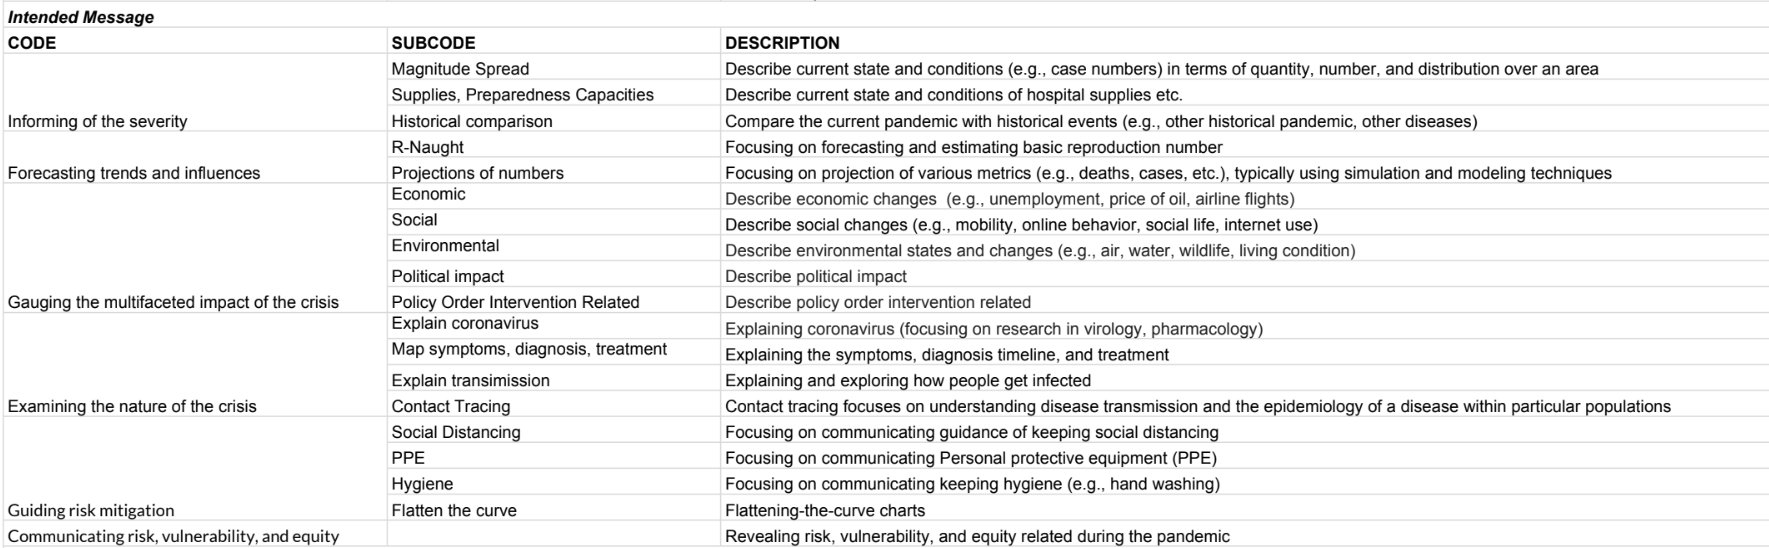
\includegraphics[width=12cm]{images/message_categories_zhang.png}
	\centering
	\caption{Ausschnitt zur Erklärung des Codebooks von Zhang ~\citep{YixuanZhang.2021}}
\end{figure}

Das Codebook beinhaltet zudem Informationen über die Visualisierungsarten (Balkendiagramm etc.) sowie entsprechende Internetquellen. Aus dem Codebook kann daher ermittelt werden, welche Datenvisualisierungen für welche Information (Nachrichtenkategorie) verwendet worden sind. Hierfür wurde im Vorfeld bereits eine Auswertung des Codebooks mittels eines eigens erstellten Jupyter Notebooks gemacht. Somit ist bekannt, welche Visualisierungsarten wie häufig für welche Nachrichtenkategorie inkl. Subkategorien verwendet worden sind (siehe Abbildung 3).


\begin{figure}[ht]
	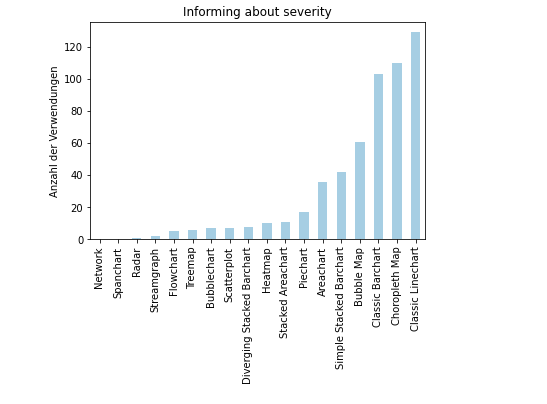
\includegraphics[width=7cm]{images/visualization_types_for_magnitude_spread.png}
	\centering
	\caption{Juypter Notebook Auswertung von verwendeten Visualisierungstypen pro Nachrichtenkategorie (Eigene Darstellung)}
\end{figure}

\clearpage
Das entsprechende Jupyter Notebook ist unter folgendem Link verfügbar \url{https://github.com/YahArt/covid-jupyter-notebook-fhgr}. Für das eigentliche Vorgehen werden \textit{teilstrukturierte Interviews} durchgeführt. Hierzu werden die Probanden zuerst danach befragt, über welche Informationen (Nachrichtenkategorie) Sie sich informieren würden. Anschliessend wird mit den Subkategorien (Subcode) die genaue Art der Information festgehalten. Zusätzlich müssen die Probanden die für sie passende Datenvisualisierung auswählen. Die Auswahl der Visualisierung pro Subkateogrie etc. ist aufgrund der Voranalyse durch das erstellte Jupyter Notebook möglich. Somit können die ersten zwei untergeordneten Forschungsfragen beantwortet werden. Um die erste untergeordnete Forschungsfrage zu beantworten, welche den Personalisierungsaspekt abdeckt, werden die Probanden darum gebeten auf bestehende Corona Dashboards zu navigieren und mittels dem \textit{think-aloud Ansatz} Ihre Gedanken möglichst offen mitzuteilen. Anschliessend werden Ihnen verschiedene Personalisierungsaspekte vorgeschlagen, welche Sie anschliessend befürworten oder ablehnen.

Dies bildet im Anschluss die Grundlage für die Erstellung eines \textit{High-Fidelity Prototypen} und schliesst somit die vorliegende Arbeit ab.


\clearpage
\subsection{Aufbau}
Die Arbeit orientiert sich wie bereits erwähnt an den ersten drei Phasen des DSR Modells von Peffers. Demzufolge ergibt sich folgende Struktur:\\

\textbf{Einleitung}
\begin{itemize}
    \item Stand der Forschung
    \item Forschungsfrage
    \item Methodisches Vorgehen\\
\end{itemize}


\textbf{Problemidentifizierung und Motivation (Identify Problem und Motivation)}
\begin{itemize}
    \item Dashboard – Ein Begriff mit Ursprung in der Automobilindustrie
    \item Die wichtigsten Komponenten und Typen eines Dashboards
    \item Überblick über die bestehenden Corona Dashboards
    \item Motivation – Erstellung eines personalisierbaren Corona Dashboards für Millennials\\
\end{itemize}

\textbf{Identifikation der Ziele (Define Objectives of a Solution)}
\begin{itemize}
    \item Erstellung des Untersuchungsinstrumentes
    \item Evaluation von Visualisierungstypen für Corona Dashboards
    \item Identifikation von relevanten Informationen
    \item Identifikation von relevanten Personalisierungsmöglichkeiten in Bezug auf Dashboards\\
\end{itemize}

\textbf{Design und Development}
\begin{itemize}
    \item Design mittels Sketching
    \item High-Fidelity Prototyp als Web Applikation\\
\end{itemize}

\textbf{Reflexion und Limitationen}

\clearpage
\section{Stand der Forschung}
Die Coronavirus-Pandemie greift seit ihrem Aufkommen im Jahr 2019 in eine Vielzahl von Lebensbereichen ein. Es ist wenig verwunderlich, dass zu einem solch einschnei-dendem Thema eine grosse Anzahl von wissenschaftlichen Publikationen erstellt worden sind. Eine Publikation untersuchte die Vielzahl von Corona Datenvisualisierungen und weist ihnen verschiedene Arten von Intentionen (Aussage über den Verlauf der Pandemie etc.) zu ~\citep{YixuanZhang.}. Weitere Quellen untersuchten speziell für das Web zugeschnittene Corona Dashboards und leiteten daraus Design Guidelines ab ~\citep{Ivankovic.2021}. Andere Studien wiederum haben sich mit der Erstellung von Dashboards für spezielle Nutzergruppen auseinandergesetzt ~\citep{Ivanov.2018}. Auch wurde bereits im Zuge einer Studie die Schwierigkeiten bei der Erstellung von Corona Dashboards aus dem Blickwinkel der eigentlichen Ersteller evaluiert ~\citep{Barbazza.}. Jedoch scheint es zum jetzigen Zeitpunkt noch keine Studie zu geben, welche die Erstellung von \textbf{personalisierbaren} Corona Dashboards für eine bestimmte Zielgruppe behandelt unter Berücksichtigung eines Nutzerzentrierten Vorgehens untersucht.

\clearpage
\bibliographystyle{apacite}
\urlstyle{rm}
\bibliography{main.bib}

\clearpage
\section*{Anhang}
\begin{table}[ht]
\begin{tabular}{@{}p{4cm}p{4cm}p{6.5cm}@{}}
\toprule
\textbf{Quelle}                                          & \textbf{Schlüsselwörter}        & \textbf{Artikel} \\ \midrule
\url{https:\\scholar.google.com}                         & covid dashboard                 & ~\citep{Dong.2020}         \\ \midrule
                                                         &                                 & ~\citep{Florez.2020}       \\ \midrule
                                                         &                                 & ~\citep{Berry.2020}        \\ \midrule
                                                         & user centered dashboards        & ~\citep{Francois.2021}     \\ \midrule
                                                         &                                 & ~\citep{Young.2020}        \\ \midrule
                                                         & customizable dasbhoards         & ~\citep{Roberts.2017}      \\ \midrule
\url{https:\\dl-acm.org}                                 & covid19 dashboard               & ~\citep{Vitale.}           \\ \midrule
                                                         & evaluating crisis dashboards    & ~\citep{Ivanov.2018}       \\ \midrule
                                                         & data dashboards                 & ~\citep{Maheshwari.}       \\ \midrule
                                                         &                                 & ~\citep{Beheshti.}         \\ \midrule
\url{https:\\google.com}                                 & covid dashboard evaluation      & ~\citep{Barbazza.}         \\ \midrule
                                                         & how user use covid19 dashboards & ~\citep{Ivankovic.2021}    \\ \bottomrule
\end{tabular}
\caption{\label{tab:research-protocol}Rechercheprotokoll (Eigene Darstellung)}
\end{table}
\clearpage


\subsection*{Zeitplan}

\begin{table}[ht]
\begin{tabular}{@{}p{13cm}p{2cm}@{}}
\toprule
\textbf{Tätigkeit}                                                                                & \textbf{Stichtag} \\ \midrule
Erstellung des Untersuchungsinstrumentes                                                          & 08.05.2022        \\ \midrule
Kapitel Einleitung fertig stellen                                                                 & 08.05.2022        \\ \midrule
Kapitel Problemidentifizierung und Motivation fertig stellen                                      & 15.05.2022        \\ \midrule
Durchführung der teilstrukturierten Interviews mit Hilfe des erstellten Untersuchungsinstrumentes & 29.05.2022        \\ \midrule
Abgabe Exposé                                                                                     & 22.05.2022        \\ \midrule
Kapitel Identifikation der Ziele fertig stellen                                                   & 05.06.2022        \\ \midrule
Implementierung Prototyp                                                                          & 26.06.2022        \\ \midrule
Kapitel Design und Development fertig stellen                                                     & 26.06.2022        \\ \midrule
Kapitel Fazit fertig stellen                                                                      & 03.07.2022        \\ \midrule
Kapitel Reflexion und Limitation fertig stellen                                                   & 10.07.2022        \\ \midrule
Korrekturlesung und Verbesserung                                                                  & 24.07.2022        \\ \midrule
Abgabe Thesis                                                                                     & 25.07.2022        \\ \bottomrule
\end{tabular}
\caption{\label{tab:time-table}Zeitplan (Eigene Darstellung)}
\end{table}


\clearpage
\section*{Eigenständigkeitserklärung}
Hiermit bestätigt der Verfasser, dass die vorliegende Arbeit selbstständig verfasst und keine anderen als die angegebenen Hilfsmittel benutzt wurden. Stellen der Arbeit, die dem Wortlaut oder dem Sinn nach anderen Werken entnommen sind, wurden unter Angaben der Quelle kenntlich gemacht.

\begin{figure}[ht]
	
\includegraphics[width=6cm]{images/signature.png}
\end{figure}
Yannick Hutter, Mels am 01. Mai 2022

\end{document}